\singlespacing
\epigraph{Everything that can be invented has been invented.}{\textit{Charles H. Duell\\ Commissioner, \\ U.S. Office of Patents (1899)}} 
\doublespace

To get started, it's probably best that you download and install TexMaker.
Within TexMaker, you should open \texttt{main.tex} as the file that you want to actually compile.
In that file you can edit anything you want, but remember that each chapter explicitly points to its own document to keep your \texttt{main.text} nice and clean. 
This chapter walks through the basics. 

Preceding text can preface section headers.
Observe how spacing is consistent, even in difficult situations that would otherwise require an inconsiderate line or section break.
By compiling the entire document, the sophisticated algorithms under the LaTeX hood have automatically rendered a consistent document.

Remember to keep your \texttt{.tex} files as well-organized as you can.
Each line in the file should correspond to one sentence.
Paragraph breaks are designated by skipped lines, and full line breaks in text are designated with two back-slashes like this.\\

See, a full line break.


\section{A basic section header}

Text goes here. 
If you don't like the epigraph above, replace it, or delete it. 
By default, new sections are numbered. 
Don't like numbers? 
Use an asterisk to remove them, like this:

\section*{Unnumbered section header}

This is now a new section. 
Importantly, unnumbered sections are not included in the table of contents.
By the way, do you see how easy it is to make the table of contents, figures, and tables?
A single line in LaTeX takes care of innumerable minutes of frustration in Word.

Need subsections? 
Easy beans.

\subsection{Here's a subsection}

\subsubsection{Sub-subsections go deeper still}

Although common convention is to halt display of sub-indices in the section header, this can be changed. 
I don't remember how to, but Google can explain. 
It's not hard, I promise.

Intermediate text is ignored in the table of contents, but the section and subsection headers are automatically included

\section{Text Formatting}

You can make words \textbf{bold} or \textit{italicized} very easily and explicitly.
As is almost always the case, LaTeX supports nested operations, so \textbf{\textit{anything}} can be modified however you want.
I like to use \texttt{mono} text for things like variables or URLs.

\section{Figures}

To include a figure in your document, you must first save the figure in a good location to which you can point LaTeX.
A figure is first defined and then populated with the graphics object, a caption, and a label.
The label is important, as it allows you to effortless refer to the specific figure from anywhere in the text withour needing to keep track of anything yourself, by referencing Figure \ref{fig:fig1} just like that.
You can control the placemenet of figures on the page by placing variables in the square brackets following the \texttt{\textbackslash begin\{figure\}} line, such as  \texttt{\textbackslash begin\{figure\}[hbt]}, where \texttt{h,b,t} designate ``here'', ``bottom'', and ``top'', respectively.
Note that in \texttt{main.tex}, I explicitly designate a graphics path, so the pointer in \texttt{includegraphics} should only require the figure name, not the full path.
Easy!

\begin{figure}[t]
\center
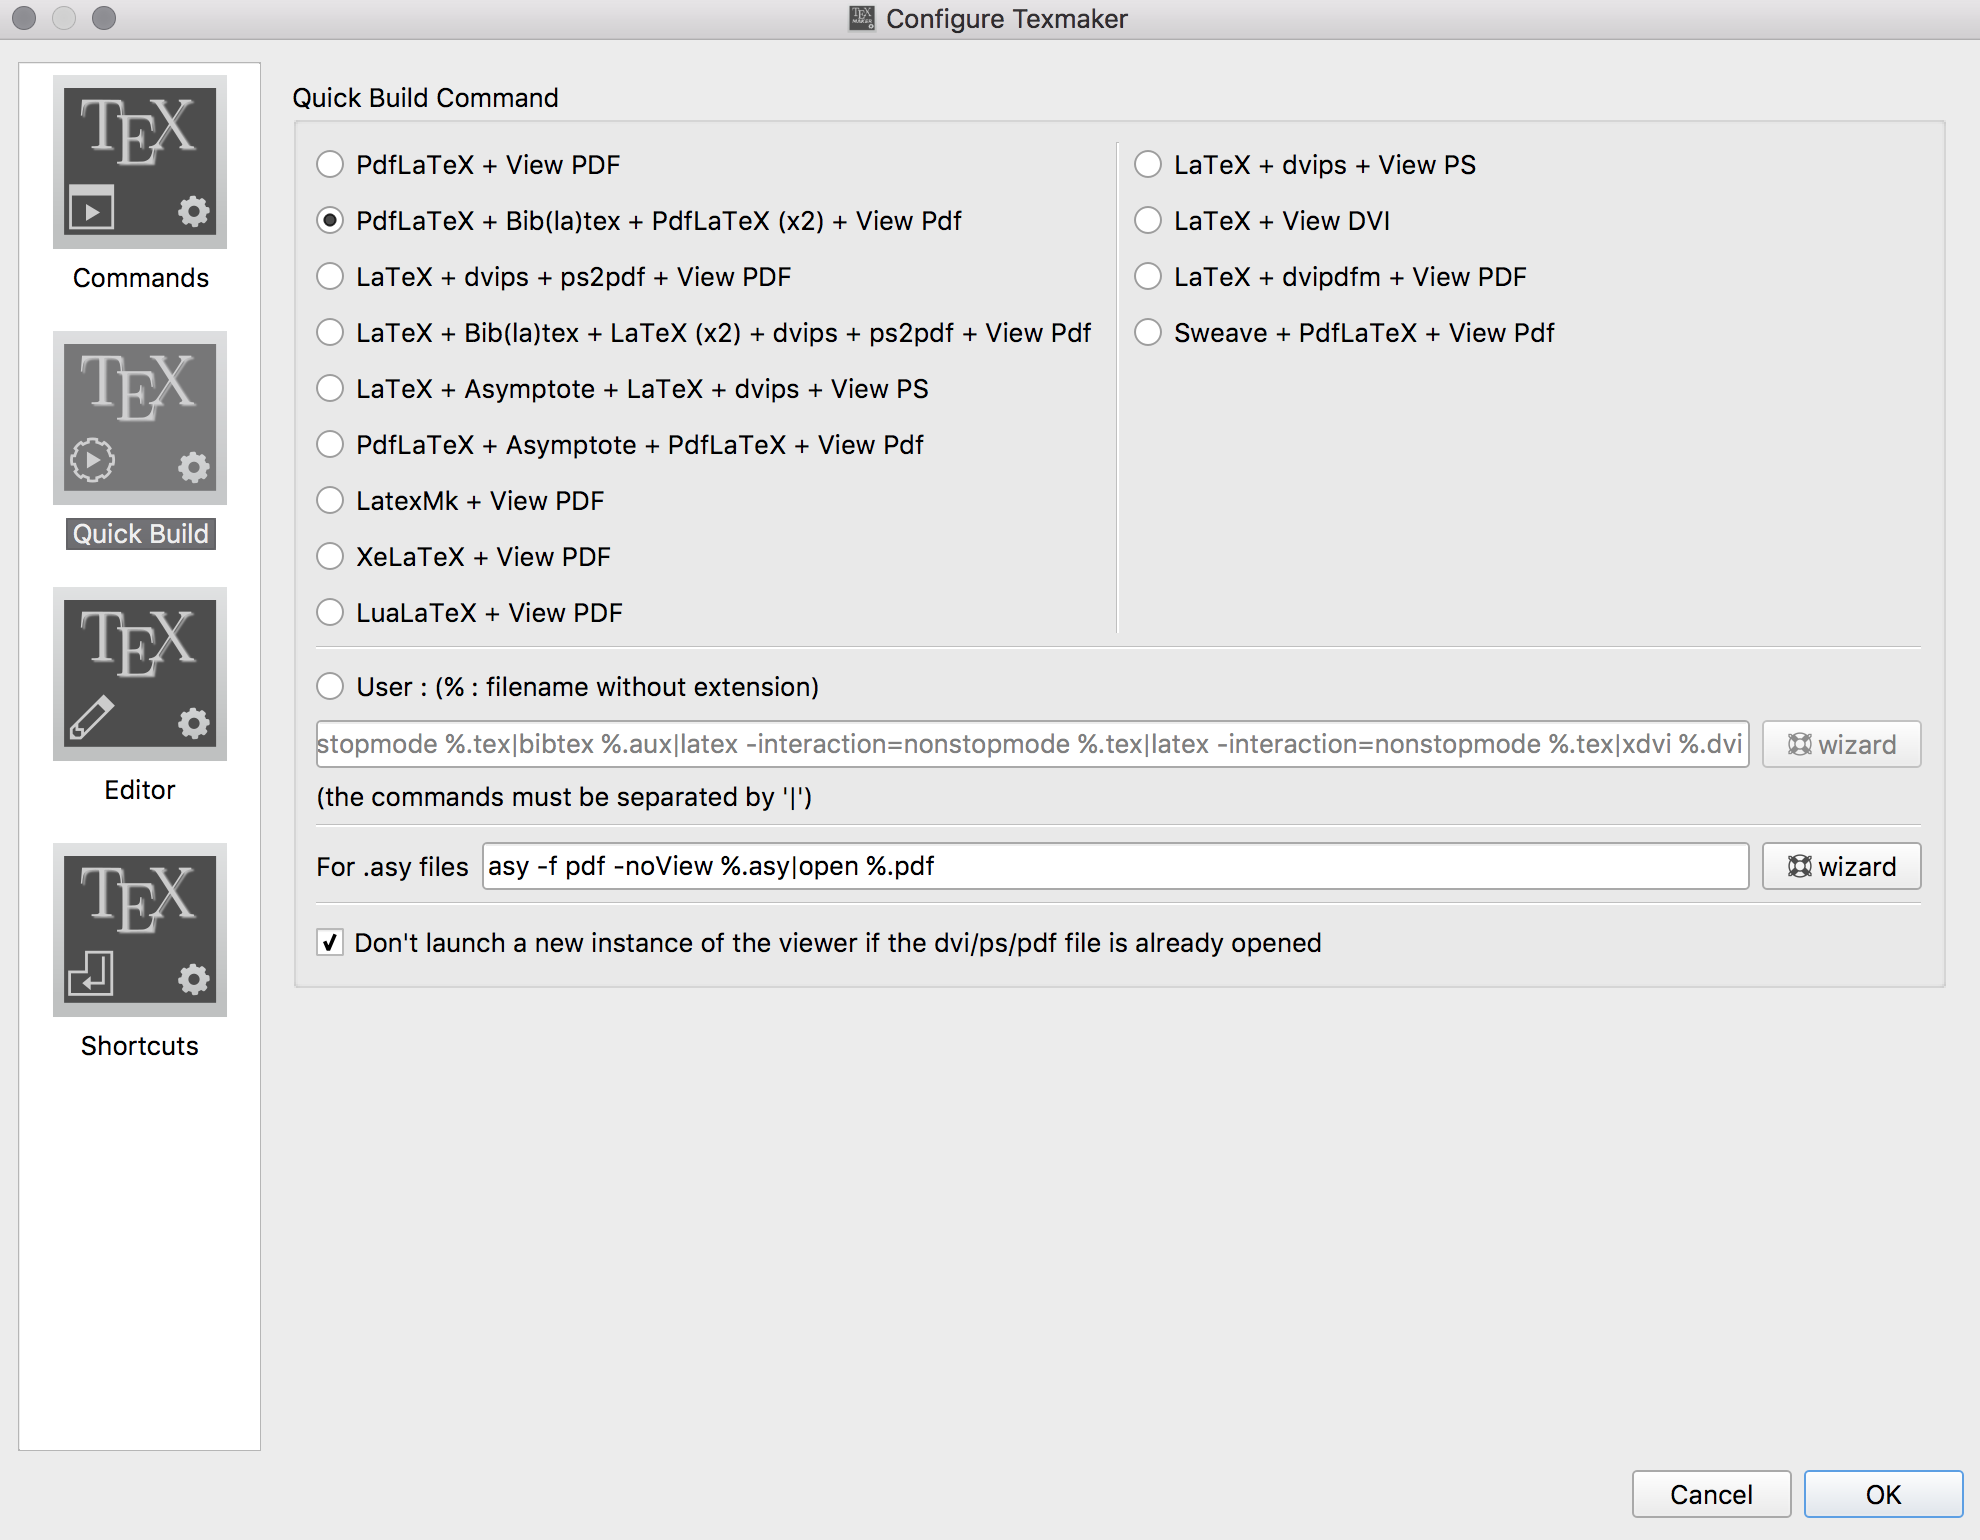
\includegraphics[width=4in]{fig1.png}
\caption{Example figure - TexMaker configuration option}
\label{fig:fig1}
\end{figure}

Pointing a document to a file on a computer when compiling is far superior to dropping the file into a document for many reasons, but risks abound. 
On one hand, this approach is elegant, because if you execute code that generates figures, you can keep the pointer the same in the LaTeX document so that each time it is compiled it will automatically load the most recent figures on your filesystem.
However, if you ever remove figures from the path, then the LaTeX pointers get confused. 
In my experience, it's a good idea to copy figures from your disk into the latex document directory rather than linking them.

\section{Tables}

Tables can become complicated quickly, but a few key properties make tables more readable than others.
The table should be top and bottom-ruled with a thicker boarder while intermediate line breaks should be used sparingly, and done with a thinner boarder.
Text should not bleed into the margins, and should be rotated onto their own page if necessary.
Just like figures, they can be referenced in the same way, like referencing Table \ref{tab:example_table}.


\begin{table}[b]
  \caption{An example table}
  \label{tab:example_table}
  \centering
  \begin{tabular}{lllllll}
    \toprule
    & \multicolumn{3}{l}{VAE} & &\\
	\cmidrule(r){2-4}
                & PC1 	        & PC2    	& LD1 		    & HCF       & Cell Count\\
    \midrule
    F value 	& 717.9		    & 8.2        &    1073 	    & 254       & 431.5 \\
    Pr ($>$ F)	&  $<$ 2e-16*    & 2.83e-4*   & $<$ 2e-16*  	& $<$ 2e-16* & $<$ 2e-16* \\
    \bottomrule
  \end{tabular}
\end{table}


\section{Equations}

Equations can obviously get very complicated, but the basic structure is to wrap your equation in a similar manner to figures and tables with a reference label, so you can reference things like Equation \ref{eq:a} or \ref{eq:vaeloss}.

\begin{equation}
\label{eq:a}
a = 10
\end{equation}

Here's an example of the pretty equation describing the loss term of my favorite deep learning model.

\begin{equation} 
\label{eq:vaeloss}
\mathcal{L}_i(x_i, \theta, \phi) = -\mathbb{E}_{z\sim q_\theta(z|x_i)}[\log p_\phi (x_i | z)] + \text{KL}(q_\theta(z|x_i)\|p(z))
\end{equation}

See Google for any specific help writing equations.
The syntax can feel like a lot, but the syntax for generating complex equations is extremely powerful and is the gold standard for mathematical writing. 


\section{Lists}

LaTeX has a myriad of mechanisms to generate lists, but the two most common are the bullet-style list and enumerated lists.

\begin{itemize}
\item Itemized lists and enumerated lists are identical except for the element's header
\item Simply replace \texttt{itemized} with \texttt{enumerated}
\end{itemize}

But, as is always good practice, multiple instances of tables, figures, or lists should be separated by some sort of text.

\begin{enumerate}
\item See, easy as that.
\item In both cases, sub-bullets are created simply by defining nested itemized or bullet lists
\begin{itemize}
\item In general, the leading characters are automatically updated for you, but can be modified any way you wish.
\begin{enumerate}
\item See Google for more examples
\end{enumerate}
\end{itemize}
\end{enumerate}

\section{Citations}

The bibliography system in LaTeX is one of its greatest features by making life immesurably easier than my previous experience with Word. 
To generate a bibliography, select the relevant documents in Mendeley or Zotero and export the selection as a \texttt{.bib} file format, which includes all necessary metadata about the citation plus a unique handle to refer to within a LaTeX document.
I have included a \texttt{bib.bib} file from a random selection of documents in the root on this project.
You can cite as many or as few as you want in the text, and LaTeX will pull them automatically and collate them into a bibliography at the end of this document, with citations made as simple as this.\cite{Lin2017}.

See the \texttt{main.tex} file to see how easy it is to point LaTeX to your bibliography.
Everything else works like magic.

\subsection{Footnotes}

I like footnotes.
I think they are fun to read and write, and give voice to the tangential thoughts of an otherwise omnipresent author.
Footnotes are easy in LaTeX, and can be used for quick references or to make a parenthetical point.\footnote{I don't have a reference, but look how easy footnotes are in LaTeX!} 
If you are a fan of judicial legal opinions or the writing of David Foster Wallace (who isn't?), then nested footnotes might be your bag.\footnote{But honestly, they're probably not a good idea for scientific writing.\footnotemark}
\footnotetext{Unless you really want to lead your reader through a long parenthetical maze of free-thinking, minimize the use of footnotes in a dissertation.\footnotemark}
\footnotetext{In fact, it's probably better that you don't use them at all}


\section{Comments}

Remember that just like computer code, you can comment out text in latex by appending a \% character in front of the line. 
This is also why keeping one sentence per line makes sense. 
A quick note on special characters in-text: because LaTeX reserves certain characters, like the percent sign, for special use, most special characters require a preceding backslash.
So things like \% and  \& need to be specifically designated. 
Google can provide a full list of special characters.

\section{Epigraphs}

I have included epigraphs for each chapter (those little quotes at the beginning).
I like them, some don't, remove them if you desire. 
Some people also don't like the Oxford comma; those people do happen to be wrong and misguided.

\section{Misspellings}

Here is where I sheepishly tuck my evangelical tail.
I admit that LaTeX does not have great support for identifying spelling or grammar mistakes.
In a pure ``what you see is what you get'' philosophy, LaTeX allows you to do whatever you want without imposing itself on how you should be doing them. 
This means it stays out of the way when you make a spelling mistake.
The solution that I find most simple is to just copy the text in the \texttt{tex} file and paste it into Word so you can go through and quickly find the little red squiggly lines.


\section{Errata}

If there is anything in this document that you would like to see modified, please let myself or the current document owner know. 
This may be hosted on github at some point for anyone to copy and easily get started with, but I will save that for a later day.

If you found this helpful, tips are accepted at the following Bitcoin wallet address:

\center

\texttt{1KTY4tQYbsdXYHNj9kHpe8UKMDEnncAaBw}

\justify


